\section{Assurances}
    The term assurances was introduced in the previous section as the name by which feedback will be known in a human-AI trust relationship. A more detailed definition and discussion is merited.

    \citet{McKnight2001-fa} alludes to this kind of feedback in an e-commerce relationship as `Web Vendor Interventions' and mentions some possible actions that might be used in that specific application. They go as far as making a diagram that indicates that these interventions could affect the `Trusting Beliefs', `Trusting Intentions', and `Trust-Related Behaviors' (see Figure \ref{fig:UserTrust}).
    
    \citet{Lillard2016-yg} coined the term `assurances' as the ability of an autonomous system to affect the user's trust, and states that it is important to note that while generally the term assurance has a positive connotation; in this setting it must encompass both positive (increasing trust) and negative (decreasing trust) feedback.

    This work is meant to be related to that of \citet{Lillard2016-yg}, but more general. Here the assurance framework is set in a more general light, although with the goal of being applied in a very similar application. Instead of treating or at least inferring that the user-autonomy trust loop is very strict and well structured, and that user trust does not take into account the institutional component proposed by \citet{McKnight2001-fa}, we re-institute the notion of institutional trust into the human-autonomy relationships.

    Regarding the relationship with the work of \citet{McKnight2001-fa}, adopt the position that besides being applied to the e-commerce industry their trust model also applies to relationships between humans and autonomy (as in \citet{Lillard2016-yg}). However, it is argued that assurances cannot directly have an affect on the user TRBs. This premise is that no autonomy (or vendor) should be able to control the TRBs of a human.

	\begin{sidewaysfigure}[htbp]
        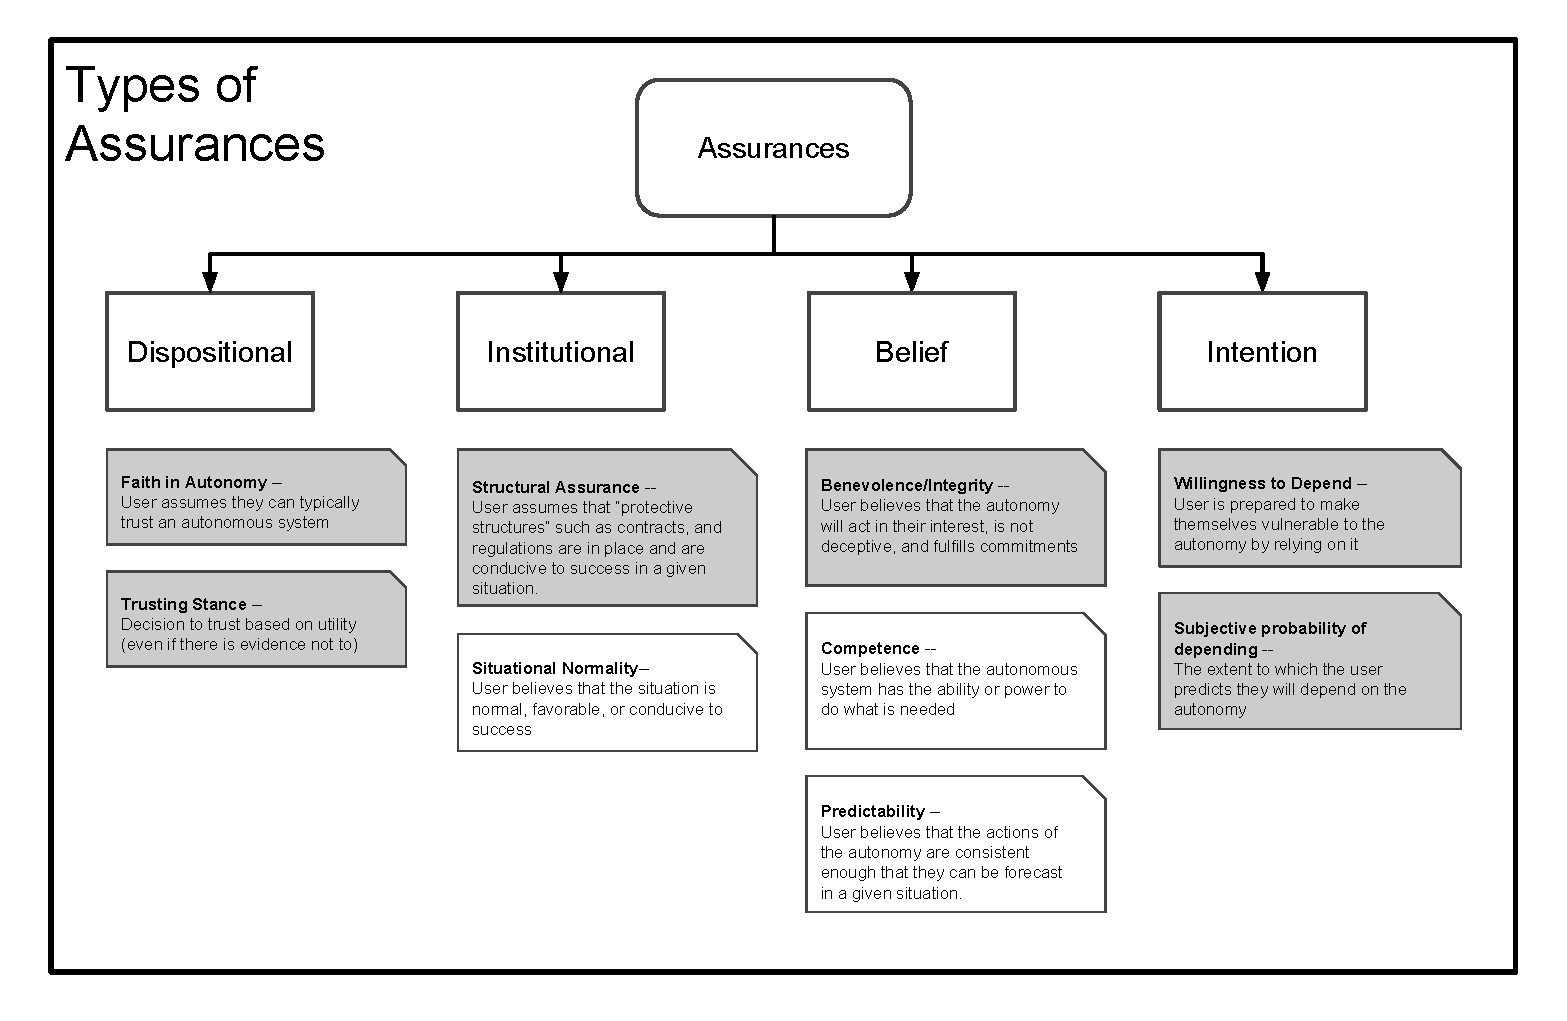
\includegraphics[width=8in]{Figures/Assurances.pdf}%
    	\caption{\textbf{Diagram delineating the possible classes of assurances, and suggesting those classes that directly apply in calibration of TRBs \ldots obviously needs to be finished \ldots}}
        \label{fig:Assurance_classes}
    \end{sidewaysfigure}

    Figure \ref{fig:Assurance_classes} shows the hierarchy of proposed assurance classes. The categories mirror those of the trust model proposed by \citet{McKnight2001-fa}, but with the emphasis on what an AI has the ability to influence. The colored boxes identify the different classes assurances. All classes are included here for completeness and generality. Although, due to practical limitations it might hypothetically possible for an AI to influence a persons general `Trusting stance' given enough time\footnote{One might imagine a AI that specifically speaks to the human about the benefits or drawbacks about trusting even though there might not be evidence to do so, similar to the role a counselor might play}, .

    Talk about the two classes of assurances: Passive and Active.

    \begin{description}
        \item [Passive:] Assurances that are not purposfully given by AI. Could be compared to non-verbal communication\ldots well not quite
        \begin{itemize}
            \item Such as success in completing the task (of course the autonomy wants to, but the outcome is independent).
            \item The way an autonomous vehicle looks when it is driving (something with weird driving habits for whatever reason might engender less trust). 
            \item 
        \end{itemize}
        \item [Active:] Assurances that are purposefully given by AI.
        \begin{itemize}
            \item Legible motion
            \item $R^2$
            \item Counter planning
            \item task similarity (to ideal task)
            \item etc.
        \end{itemize}
    \end{description}

    Each type of assurance can be given in passive or active ways. Perhaps they can be treated analogously to actions and words, specifically `actions speak louder than words' or `passive assurances speak louder than active ones'. The point is that actually doing something instead of just saying it will do a lot for bolstering trust. What is better saying: I can do this, or actually doing it?

    However, for the case of calibrating TRBs it is proposed that the classes should be constrained as shown in Figure \ref{fig:Assurance_classes}. An AI that is trying to calibrate the TRBs of a user (as opposed to just influencing them to its own benefit), should not actively try to convice the user that it should have faith in autonomy, or that it is benevolent, or that the institutional system should be trusted.

    Due to the nature of trust a single assurance might be targeted at influencing the competence dimension of trust, but it will likely also have affects on other dimensions. As an example an assurance aimed at influencing Predictability may also have an affect on the Probability of Depending.

    Besides being difficult to separate, each user is different. Thus no assurance will work identically when given to two separate users.

    \textbf{I am not sure how I want this argument to go, I want to highlight that it is theoretically possible to have some affect on each of these attributes, but that some are more practical. Two main things need to be considred 1) time-scale (how long will it take to make a noticeable change), and 2) what SHOULD be influenced in order to appropriately calibrate TRBs (it probably isn't acceptable to lie in order to manipulate a user's trust)?}
    


